% Source-coordinate reconstruction. Edit named defaults or copy this entire composition.
\studiodeclarefield{graphic-1}{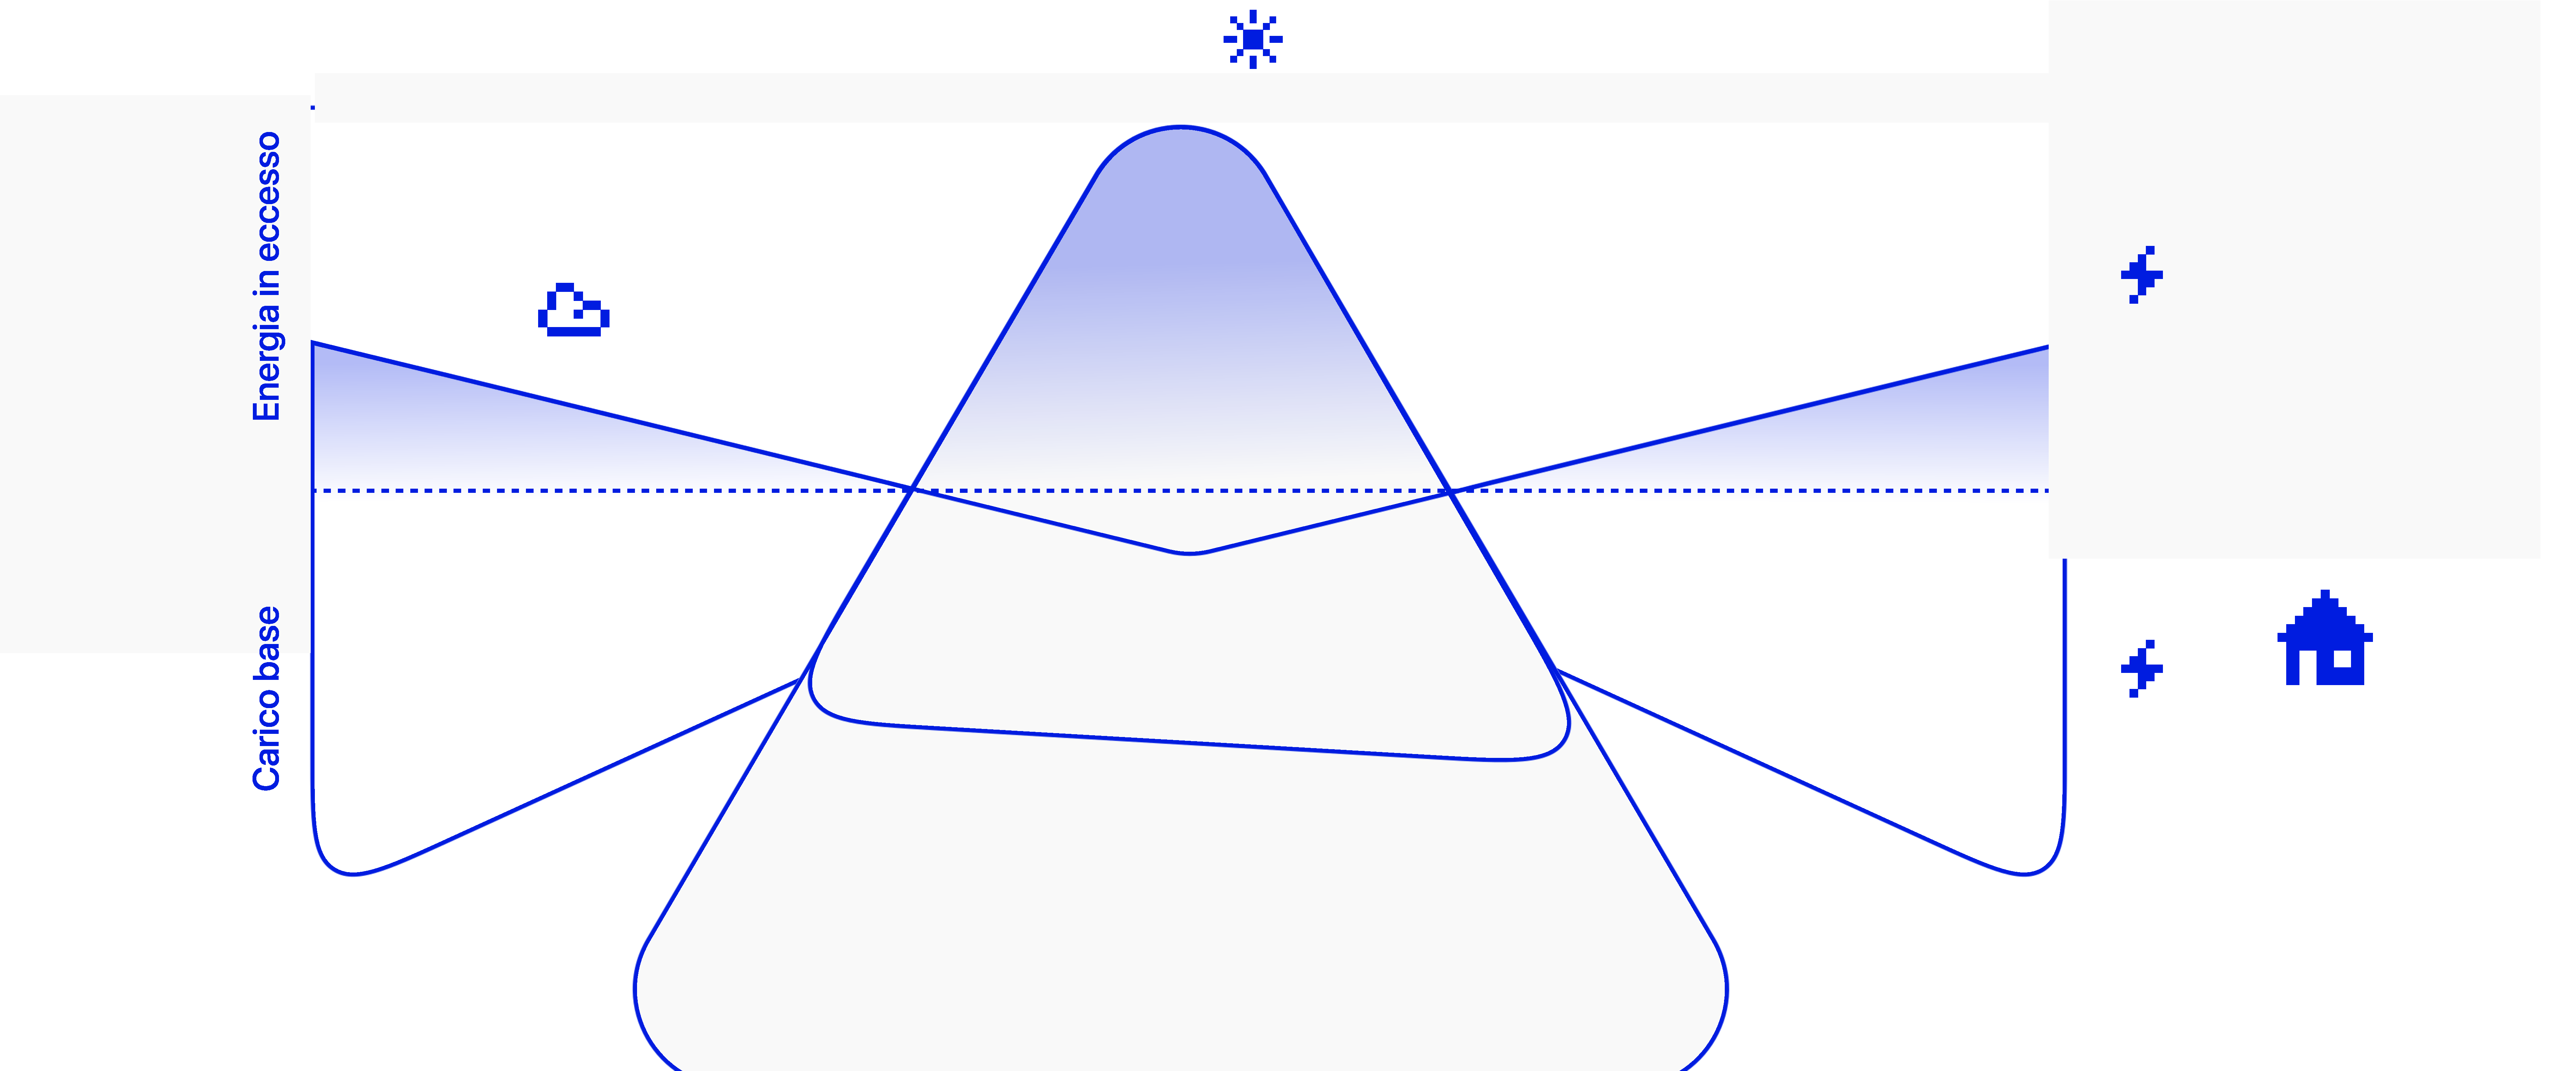
\includegraphics[width=3550\studiounit]{images/studio/collection/figma-0525-part-01.pdf}}
\studiodeclarefield{title}{Energy consumption}
\studiodeclarefield{text-2}{Night}
\studiodeclarefield{text-3}{Energy produced}
\studiodeclarefield{text-4}{Noon}
\studiodeclarefield{text-5}{Day}
\studiodeclarefield{text-6}{Mine\\bitcoin}
\studiodeclarefield{text-7}{Sell to\\the grid}
\studiodeclarefield{text-8}{Wind}
\studiodeclarefield{text-9}{Solar}
\studioapplyfields
\studiomeasuredcanvas{3556}{2000}{diagram-annotated-energy}{studio-paper}{
\studiomeasuredtext{title}{1195.81}{227.41}{1165.41}{170.41}{113.04}{131.126}{\color{bitpolito}\bfseries\centering}{\studiofield{title}}
\studiographfield{graphic-1}{0}{524}{3550}{1476}{}{}
\path[fill=studio-paper,draw=none,line width=1\studiounit] (1258.91,1201.45)--(1993.32,1202)--(2324.92,1760.05)--(931.203,1761.72)--(1258.91,1201.45)--cycle;
\path[fill=studio-paper,draw=none,line width=1\studiounit] (434.359,1259.86)--(1208.83,1272.66)--(924.527,1759.49)--(434.359,1759.49)--(434.359,1259.86)--cycle;
\path[fill=studio-paper,draw=none,line width=1\studiounit] (3038.2,1272.66)--(2044.51,1272.66)--(2328.82,1759.49)--(2818.98,1759.49)--(3038.2,1272.66)--cycle;
\path[fill=bitpolito,draw=none,line width=1\studiounit] (431.023,1765.61)--(433.805,1765.61)--(433.805,586.649)--(431.023,586.649)--(428.242,586.649)--(428.242,1765.61)--(431.023,1765.61)--cycle (431.023,561.612)--(414.962,589.431)--(447.085,589.431)--(431.023,561.612)--cycle;
\path[fill=bitpolito,draw=none,line width=1\studiounit] (431.023,1762.83)--(431.023,1765.61)--(2798.4,1765.61)--(2798.4,1762.83)--(2798.4,1760.05)--(431.023,1760.05)--(431.023,1762.83)--cycle (2823.44,1762.83)--(2795.62,1746.77)--(2795.62,1778.89)--(2823.44,1762.83)--cycle;
\path[fill=studio-paper,draw=none,line width=1\studiounit,rounded corners=0\studiounit] (682.5,1765.61) rectangle (2664.31,2105);
\path[fill=studio-paper,draw=none,line width=1\studiounit,rounded corners=0\studiounit] (682.5,1765.61) rectangle (2664.31,2105);
\studiomeasuredtext{text-2}{377.266}{1826.78}{146.377}{61.5733}{46.9733}{54.4891}{\color{bitpolito}}{\studiofield{text-2}}
\studiomeasuredtext{text-3}{258.906}{464.281}{381.584}{70.6123}{46.9733}{54.4891}{\color{bitpolito}}{\studiofield{text-3}}
\studiomeasuredtext{text-4}{705.987}{1826.78}{1934.84}{61.5733}{46.9733}{54.4891}{\color{bitpolito}\centering}{\studiofield{text-4}}
\studiomeasuredtext{text-5}{2659.39}{1826.19}{173.098}{63.0913}{48.5333}{56.2987}{\color{bitpolito}}{\studiofield{text-5}}
\path[fill=none,draw=bitpolito,line width=5.56376\studiounit] (2862,1744)--(2862,1213);
\path[fill=none,draw=bitpolito,line width=5\studiounit] (2865,1742.5)--(2832,1742.5);
\path[fill=none,draw=bitpolito,line width=5\studiounit] (2865,1213)--(2832,1213);
\path[fill=none,draw=bitpolito,line width=5\studiounit] (2865,1183)--(2832,1183);
\path[fill=none,draw=bitpolito,line width=5\studiounit] (2865,700)--(2832,700);
\path[fill=none,draw=bitpolito,line width=5.56376\studiounit] (2862,1183)--(2862,700);
\studiomeasuredtext{text-6}{3123.19}{989.355}{358.183}{146.478}{56.3733}{65.3931}{\color{bitpolito}}{\studiofield{text-6}}
\path[fill=bitpolito,draw=none,line width=1\studiounit] (3150,904.152)--(3161.81,904.152)--(3161.81,916.412)--(3150,916.412)--(3150,904.152)--cycle;
\path[fill=bitpolito,draw=none,line width=1\studiounit] (3161.8,868.742)--(3173.61,868.742)--(3173.61,880.548)--(3161.8,880.548)--(3161.8,868.742)--cycle;
\path[fill=bitpolito,draw=none,line width=1\studiounit] (3161.8,880.547)--(3173.61,880.547)--(3173.61,892.352)--(3161.8,892.352)--(3161.8,880.547)--cycle;
\path[fill=bitpolito,draw=none,line width=1\studiounit] (3161.8,892.352)--(3173.61,892.352)--(3173.61,904.157)--(3161.8,904.157)--(3161.8,892.352)--cycle;
\path[fill=bitpolito,draw=none,line width=1\studiounit] (3161.8,904.152)--(3173.61,904.152)--(3173.61,916.412)--(3161.8,916.412)--(3161.8,904.152)--cycle;
\path[fill=bitpolito,draw=none,line width=1\studiounit] (3173.61,809.262)--(3185.87,809.262)--(3185.87,821.067)--(3173.61,821.067)--(3173.61,809.262)--cycle;
\path[fill=bitpolito,draw=none,line width=1\studiounit] (3173.61,832.875)--(3185.87,832.875)--(3185.87,844.68)--(3173.61,844.68)--(3173.61,832.875)--cycle;
\path[fill=bitpolito,draw=none,line width=1\studiounit] (3173.61,844.672)--(3185.87,844.672)--(3185.87,856.477)--(3173.61,856.477)--(3173.61,844.672)--cycle;
\path[fill=bitpolito,draw=none,line width=1\studiounit] (3173.61,856.48)--(3185.87,856.48)--(3185.87,868.74)--(3173.61,868.74)--(3173.61,856.48)--cycle;
\path[fill=bitpolito,draw=none,line width=1\studiounit] (3173.61,868.742)--(3185.87,868.742)--(3185.87,880.548)--(3173.61,880.548)--(3173.61,868.742)--cycle;
\path[fill=bitpolito,draw=none,line width=1\studiounit] (3173.61,880.547)--(3185.87,880.547)--(3185.87,892.352)--(3173.61,892.352)--(3173.61,880.547)--cycle;
\path[fill=bitpolito,draw=none,line width=1\studiounit] (3173.61,892.352)--(3185.87,892.352)--(3185.87,904.157)--(3173.61,904.157)--(3173.61,892.352)--cycle;
\path[fill=bitpolito,draw=none,line width=1\studiounit] (3173.61,904.152)--(3185.87,904.152)--(3185.87,916.412)--(3173.61,916.412)--(3173.61,904.152)--cycle;
\path[fill=bitpolito,draw=none,line width=1\studiounit] (3173.61,916.414)--(3185.87,916.414)--(3185.87,928.219)--(3173.61,928.219)--(3173.61,916.414)--cycle;
\path[fill=bitpolito,draw=none,line width=1\studiounit] (3185.88,809.262)--(3197.68,809.262)--(3197.68,821.067)--(3185.88,821.067)--(3185.88,809.262)--cycle;
\path[fill=bitpolito,draw=none,line width=1\studiounit] (3185.88,821.062)--(3197.68,821.062)--(3197.68,832.868)--(3185.88,832.868)--(3185.88,821.062)--cycle;
\path[fill=bitpolito,draw=none,line width=1\studiounit] (3185.88,832.875)--(3197.68,832.875)--(3197.68,844.68)--(3185.88,844.68)--(3185.88,832.875)--cycle;
\path[fill=bitpolito,draw=none,line width=1\studiounit] (3185.88,844.672)--(3197.68,844.672)--(3197.68,856.477)--(3185.88,856.477)--(3185.88,844.672)--cycle;
\path[fill=bitpolito,draw=none,line width=1\studiounit] (3185.88,856.48)--(3197.68,856.48)--(3197.68,868.74)--(3185.88,868.74)--(3185.88,856.48)--cycle;
\path[fill=bitpolito,draw=none,line width=1\studiounit] (3185.88,868.742)--(3197.68,868.742)--(3197.68,880.548)--(3185.88,880.548)--(3185.88,868.742)--cycle;
\path[fill=bitpolito,draw=none,line width=1\studiounit] (3185.88,904.152)--(3197.68,904.152)--(3197.68,916.412)--(3185.88,916.412)--(3185.88,904.152)--cycle;
\path[fill=bitpolito,draw=none,line width=1\studiounit] (3197.68,797)--(3209.49,797)--(3209.49,809.259)--(3197.68,809.259)--(3197.68,797)--cycle;
\path[fill=bitpolito,draw=none,line width=1\studiounit] (3197.68,809.262)--(3209.49,809.262)--(3209.49,821.067)--(3197.68,821.067)--(3197.68,809.262)--cycle;
\path[fill=bitpolito,draw=none,line width=1\studiounit] (3197.68,821.062)--(3209.49,821.062)--(3209.49,832.868)--(3197.68,832.868)--(3197.68,821.062)--cycle;
\path[fill=bitpolito,draw=none,line width=1\studiounit] (3197.68,856.48)--(3209.49,856.48)--(3209.49,868.74)--(3197.68,868.74)--(3197.68,856.48)--cycle;
\path[fill=bitpolito,draw=none,line width=1\studiounit] (3197.68,904.152)--(3209.49,904.152)--(3209.49,916.412)--(3197.68,916.412)--(3197.68,904.152)--cycle;
\path[fill=bitpolito,draw=none,line width=1\studiounit] (3197.68,916.414)--(3209.49,916.414)--(3209.49,928.219)--(3197.68,928.219)--(3197.68,916.414)--cycle;
\path[fill=bitpolito,draw=none,line width=1\studiounit] (3209.48,809.262)--(3221.29,809.262)--(3221.29,821.067)--(3209.48,821.067)--(3209.48,809.262)--cycle;
\path[fill=bitpolito,draw=none,line width=1\studiounit] (3209.48,856.48)--(3221.29,856.48)--(3221.29,868.74)--(3209.48,868.74)--(3209.48,856.48)--cycle;
\path[fill=bitpolito,draw=none,line width=1\studiounit] (3209.48,892.352)--(3221.29,892.352)--(3221.29,904.157)--(3209.48,904.157)--(3209.48,892.352)--cycle;
\path[fill=bitpolito,draw=none,line width=1\studiounit] (3209.48,904.152)--(3221.29,904.152)--(3221.29,916.412)--(3209.48,916.412)--(3209.48,904.152)--cycle;
\path[fill=bitpolito,draw=none,line width=1\studiounit] (3221.28,797)--(3233.54,797)--(3233.54,809.259)--(3221.28,809.259)--(3221.28,797)--cycle;
\path[fill=bitpolito,draw=none,line width=1\studiounit] (3221.28,809.262)--(3233.54,809.262)--(3233.54,821.067)--(3221.28,821.067)--(3221.28,809.262)--cycle;
\path[fill=bitpolito,draw=none,line width=1\studiounit] (3221.28,844.672)--(3233.54,844.672)--(3233.54,856.477)--(3221.28,856.477)--(3221.28,844.672)--cycle;
\path[fill=bitpolito,draw=none,line width=1\studiounit] (3221.28,856.48)--(3233.54,856.48)--(3233.54,868.74)--(3221.28,868.74)--(3221.28,856.48)--cycle;
\path[fill=bitpolito,draw=none,line width=1\studiounit] (3221.28,868.742)--(3233.54,868.742)--(3233.54,880.548)--(3221.28,880.548)--(3221.28,868.742)--cycle;
\path[fill=bitpolito,draw=none,line width=1\studiounit] (3221.28,880.547)--(3233.54,880.547)--(3233.54,892.352)--(3221.28,892.352)--(3221.28,880.547)--cycle;
\path[fill=bitpolito,draw=none,line width=1\studiounit] (3221.28,892.352)--(3233.54,892.352)--(3233.54,904.157)--(3221.28,904.157)--(3221.28,892.352)--cycle;
\path[fill=bitpolito,draw=none,line width=1\studiounit] (3221.28,904.152)--(3233.54,904.152)--(3233.54,916.412)--(3221.28,916.412)--(3221.28,904.152)--cycle;
\path[fill=bitpolito,draw=none,line width=1\studiounit] (3233.55,809.262)--(3245.35,809.262)--(3245.35,821.067)--(3233.55,821.067)--(3233.55,809.262)--cycle;
\path[fill=bitpolito,draw=none,line width=1\studiounit] (3233.55,821.062)--(3245.35,821.062)--(3245.35,832.868)--(3233.55,832.868)--(3233.55,821.062)--cycle;
\path[fill=bitpolito,draw=none,line width=1\studiounit] (3233.55,832.875)--(3245.35,832.875)--(3245.35,844.68)--(3233.55,844.68)--(3233.55,832.875)--cycle;
\path[fill=bitpolito,draw=none,line width=1\studiounit] (3233.55,844.672)--(3245.35,844.672)--(3245.35,856.477)--(3233.55,856.477)--(3233.55,844.672)--cycle;
\path[fill=bitpolito,draw=none,line width=1\studiounit] (3233.55,868.742)--(3245.35,868.742)--(3245.35,880.548)--(3233.55,880.548)--(3233.55,868.742)--cycle;
\path[fill=bitpolito,draw=none,line width=1\studiounit] (3233.55,880.547)--(3245.35,880.547)--(3245.35,892.352)--(3233.55,892.352)--(3233.55,880.547)--cycle;
\path[fill=bitpolito,draw=none,line width=1\studiounit] (3233.55,892.352)--(3245.35,892.352)--(3245.35,904.157)--(3233.55,904.157)--(3233.55,892.352)--cycle;
\path[fill=bitpolito,draw=none,line width=1\studiounit] (3245.35,821.062)--(3257.16,821.062)--(3257.16,832.868)--(3245.35,832.868)--(3245.35,821.062)--cycle;
\path[fill=bitpolito,draw=none,line width=1\studiounit] (3245.35,832.875)--(3257.16,832.875)--(3257.16,844.68)--(3245.35,844.68)--(3245.35,832.875)--cycle;
\path[fill=bitpolito,draw=none,line width=1\studiounit] (2863.49,964.43)--(2863.49,967.212)--(2999.8,967.212)--(2999.8,964.43)--(2999.8,961.648)--(2863.49,961.648)--(2863.49,964.43)--cycle (3024.84,964.43)--(2997.02,948.369)--(2997.02,980.491)--(3024.84,964.43)--cycle;
\studiomeasuredtext{text-7}{3101.15}{1529}{249.874}{146.344}{57.1867}{66.3365}{\color{bitpolito}}{\studiofield{text-7}}
\path[fill=bitpolito,draw=none,line width=1\studiounit] (2863.49,1504.11)--(2863.49,1506.9)--(2999.8,1506.9)--(2999.8,1504.11)--(2999.8,1501.33)--(2863.49,1501.33)--(2863.49,1504.11)--cycle (3024.84,1504.11)--(2997.02,1488.05)--(2997.02,1520.17)--(3024.84,1504.11)--cycle;
\studiomeasuredtext{text-8}{560.965}{929.141}{184.615}{74.4747}{56.3667}{65.3853}{\color{bitpolito}}{\studiofield{text-8}}
\studiomeasuredtext{text-9}{1494.63}{553.02}{197.768}{75.7175}{58.2427}{67.5615}{\color{bitpolito}}{\studiofield{text-9}}
}
